\maketitle
%\thispagestyle{fancy}
\section{Introduction}

This is the full report.

\subsection{Overview of the Swarm system}

The Swarm mechanism is defined in \cite{book-of-swarm}.

The mechanism underlying the Swarm protocol can be understood as comprising three sets of agents exchanging financial instruments:
\begin{itemize}
  \item Users, a.k.a.~storage clients;
  \item The Swarm system, comprising (a) its set of smart contracts (deployed on Gnosis Chain) and (b), the p2p network considered as an opaque blob with which data can be exchanged;
  \item Node operators, a.k.a.~storage providers.
\end{itemize}
Storage clients and storage providers do not trade with one another directly; rather, their trade is mediated by the Swarm system accounts.
%
On the demand side, users buy storage quotas from the \emph{postage stamp} contract via a posted price mechanism. This component of the system is out of scope for our study.

\subsection{Overview of the Swarm redistribution mechanism}

\begin{itemize}
  \item The redistribution mechanism is governed by the Stake Registry and Redistribution contracts.
  \item The network revenue is calculated by the Price Oracle and Postage contracts at each epoch.
  %
  The computation occurs when the Redistribution contract calls into the Postage contract to query the reward pot.
  %
  We treat these contracts largely as a black box (but see \S\ref{estimation}).
  \item 
    NOs may purchase \emph{shares} by calling the \code{stakeUpdate} function in the stake registry.
    %
    In the Book of Swarm and related literature, this operation is called \emph{depositing} or \emph{topping up stake}.
    %
    In this study, we prefer the term \emph{share} as we believe this gives a more accurate mental model of what entering into this position entails.

    Prior to SWIP-19, share balances were associated to an overlay address.
    %
    Post SWIP-19, balances are associated to a Gnosis chain address together with a derived overlay address.
    %
    That is, after these changes, each Gnosis chain address is associated to a unique share balance, instead of possibly several keyed by different overlay addresses derived using different nonces.

  \item
    Prior to SWIP-20, shares were priced at a static value $c$.
    %
    The precise value of $c$ does not matter for the dynamics (except for integer division problems); making $c$ smaller just corresponds to doing a stock split.
    %
    We adopt the convention $c=1$ PLUR, which matches how balances were tracked in the stake registry implementation (pre SWIP-20).

  \item
    Nodes are divided up into \emph{replication neighbourhoods} or \emph{bins} according to the first $D$ bits of their overlay address, where $D$ is a number determined locally by the amount of data being stored on the platform.
    %
    At time of writing, $D=11$.
    %
    Since in this study, we will assume that $D$ is a global constant, we don't need to go into details of what happens when $D$ changes.

  \item
    Time is divided into \emph{rounds} or \emph{epochs} of 152 Gnosis chain blocks --- targeting 12 minutes 40 seconds.
    %
    Each epoch, a bin is selected uniformly at random (using what randomness?).
    %
    NOs belonging to that bin may participate in the revenue sharing system during that epoch if they satisfy a few additional conditions:
    \begin{enumerate}
      \item They have not purchased additional shares within the past 2 epochs.
      \item They are not \emph{frozen} as a penalty for a consensus fault. Freezing penalties last for about 1 day.
      \item They have shares in excess of a minimum threshold $\tau$. For the versions under consideration in this study, $\tau=10$ BZZ.
    \end{enumerate}

  \item
    To participate in the revenue sharing system, nodes must submit storage proofs during a \emph{commit} and \emph{reveal} phases (the first and second quarters of an epoch --- 38 blocks, or 3 minutes 10 seconds each).
    %
    Commits are checked for agreement in a rudimentary consensus system.
    
    In the final \emph{claim} phase, any entity can call the \code{claim()} function of the redistribution contract.
    %
    This function randomly selects a node from among those that successfully submitted a commit and reveal in the previous phases, with probability weighted by the share balance of that node.
    %
    The selected node receives the full network reward for that round.

  \item
    Network revenue and share prices are both denominated in BZZ tokens.

\end{itemize}

\subsection{Scope}

In our study, we focus only on the procurement auction side of the mechanism, which governs the relationship between storage providers and the Swarm system.
%
The demand-side part of the relationship, governing the relationship between storage clients and the Swarm system, is out of scope.


\paragraph{Versions}
Our study is based on version 0.8.6 of the storage incentives contracts.
%
Since this version only introduced an update to the redistribution contract that is out of scope of the model, our model applies equally well to the versions of contracts deployed at version 0.6.0 (or version 0.4.0 in the case of the stake registry).

\subsection{Assumptions}
Stationarity, no neighbourhood splits. 

No delays (there ought to be a delay between topping up stake and being able to claim).

We didn't get into considering a lot of different competitive strategies.

\paragraph{Storage service}

On the supply side, node operators (henceforth NOs) provide a fixed service to the system, storing the data chunks delivered into their neighbourhood.
%
For simplicity, we hence assume that an NO's decision space surrounding this service is simply a binary: the service is either on or off during any given epoch.
%
We also assume that whenever the service is on, the NO remains in consensus with the rest of the neighbourhood; that is, slashing over safety failures is not considered.
%
Intermediate strategies, where service is provided only for a subset of chunks, are out of scope.

We assume there is no liveness or safety risk; nodes are inactive if they choose to be, and if they are active, they are always in consensus. (This part isn't actually true in the real Swarm. This means the changes made in the v0.8.6 upgrade of the storage incentives are out of scope for our model.)

\subsection{Recommendations}

\begin{itemize}
  \item
    As the network grows into the petabyte range, small NO operations such as a single laptop become unviable because of risk of ruin.
    %
    If demand for Swarm revenue share remains robust, the emergence of stake pools or liquid stake solutions is inevitable.

    The Swarm community should consider what staking pools might look like and whether the core protocol should be changed to either directly support stake pools or facilitate community-led initiatives.

  \item
    We have established that the lack of opportunities to reallocate stake is a barrier to economic efficiency.
    %
    Swarm should introduce more reallocation opportunities --- in particular, opportunities to exit stake positions --- so that they have an opportunity to undergo real price discovery.

  \item
    The Swarm community should consider how it wishes to prioritise the tradeoff between replication rate (and other QoS) targets and growth targets (sales or revenue).

\end{itemize}

\subsection{Notation}

\paragraph{Addresses}

The set of agents is denoted $\Overlay$.
%
It can be realised as a set of \emph{overlay addresses}, for example, $\Overlay \cong \mathbb{F}_2^{256}$.

The set of overlay addresses is divided into a set $\Bins$ of \emph{bins}.
%
In \cite{book-of-swarm}, these are also called \emph{neighbourhoods}; we prefer the term `bins' because it is shorter and because neighbourhoods can also be of various different sizes.
%
We are given a surjective map $\bin:\Overlay\rightarrow\Bins$ that takes an overlay address to the bin to which it belongs.
%
The fibre of $\bin$ over a bin $\nu\in\Bins$ is denoted $\Overlay_\nu$.

In deployments, we have $\Bins\cong \mathbb{F}_2^D$ and the function $\bin$ is projection on the first $D$ bits, where $D$ is a network-wide dynamic variable called the \emph{network (log-)radius}.
%
For any $\nu\in\Bins$, we can then identify $\Overlay_\nu\simeq\mathbb{F}_2^{256-D}$ by projecting out the first $D$ bits.


\paragraph{Balances} Balances are presumed to be non-negative real numbers, i.e.~elements of $\uR := [0,\infty)$.

\paragraph{Summation}
Fix the following notation for summation over subsets of indices:
\begin{itemize}
  \item if $x\in \mathbb{R}^I$ is a vector of finite length, write $\sum:=\sum_I:\R^I\rightarrow\R$ for the sum of the coordinates. On $\uR^I$ this coincides with the 1-norm.
  \item If $J\subseteq I$ is a subset, write $\sum_J$ for the composite $\R^I\stackrel{\pi_J}{\rightarrow}\R^J\stackrel{\sum}{\rightarrow}\R$, that is, summation over the coordinates in $J$.
  \item If $i\in I$ is a single element, write also $\sum_{\hat{i}}$ as a shorthand for $\sum_{I\setminus\{i\}}$.
  \item If $M\leq N$ are natural numbers and $x\in\R^{\Overlay\times N}$, write $x_{\leq M}\in \uR^{\Overlay\times M}$ for the projection on the first $M$ terms.
\end{itemize}



\newpage
%%%%%%%%%%%%%%%%%%%%%%%%%%%%%%%%%%%%%%%%%%%%%%%%%%%%%%%%%%%%%%%%%%%%%%%%%%%%%%%

\section{Objectives of the system design}

The objectives of the redistribution mechanism:
\begin{itemize}
  \item Decentralisation
  \item Growth
  \item Sybil resistance (of the redistribution mechanism)
  \item Safety (of the chunk index)
\end{itemize}

\subsection{Decentralisation}

Decentralisation is usually a primary objective of blockchain-based services.
%
Decentralisation can be measured in terms of the difficulty by which an adversary can unilaterally control aspects of the system.

In markets, centralisation arises in the exercise of \emph{market power}.
%
Hence, centralisation occurs as a result of market share concentration.
%
Therefore, measures of concentration of a distribution can be used as a proxy for assessing market power.

In US anti-trust legislation, the Herfindahl-Hirschman index ($L^2$ norm) is used as a measure of concentration.
%
We advocate the use of Shannon entropy because of its composition rule.

Which distributions do we want to track in Swarm?
%
\begin{itemize}
  \item The number of active nodes in a neighbourhood. This controls the replication rate.
  \item The distribution of equity within a neighbourhood.
  %
  Concentration of equity at one node gives that node consensus power over the state of the reserve, which could be used for censorship.
  %
  A highly concentrated equity pool may also indicate a trend towards consolidation and hence reduced replication rate. 
  %
  If equity is allocated efficiently, this may also give an indication of differing operating costs.
  \item The distribution of equity across neighbourhoods. We expect equity to be balanced across neighbourhoods in equilibrium, since all neighbourhoods have equal earning potential. A non-uniform distribution therefore indicates a market inefficiency.
  \item Distribution of node count and per-neighbourhood equity by controlling entity. 
  %
  This depends on identifying and labelling addresses by owner, which is prone to errors and can be gamed, but still can be somewhat informative.
  %
  Concentration of control could indicate censorship power.
  \item In order to control prices of Swarm storage (e.g.~pushing up the price to a monopoly rate), a would-be monopolist must control the average replication rate.
  %
  If the monopolist manages to acquire enough equity to make entry unprofitable, he can achieve this, especially if reallocations of stake between nodes is possible.
\end{itemize}

\subsection{Growth and efficiency}

Broadly speaking, economic efficiency means that resources are allocated where they can be deployed most productively.
%
That is, efficient allocations are those that optimise economic growth.
%
The Swarm network maintains an internal state that controls the distribution of revenue for the storage service; this redistribution is efficient if it is optimised for growth of the demand serviced, given fixed exogenous world state and constraints on the quality of service --- most essentially for us, the replication rate $q\geq 4$.
%
All other things being equal, demand tends higher when prices are lower, so an equivalent goal is the optimisation of price at the target replication rate.

In our model of the Swarm storage service, nodes are simply either active or inactive --- for simplicity, we are not taking into account any gradations in service quality (such as retrieval latency and bandwidth).
%
An efficient allocation of Swarm revenue share would allow the NOs with lowest costs to become active, driving those with higher costs out of business and allowing the cost savings to be passed onto customers in the form of lower price per replica.



\begin{comment}
Since for the purposes of this work, the service provided by each Swarm node is assumed to be of constant quality --- it's either on or off --- profit margins, and hence productivity, of a node operator, depend only on operating costs.
%
On the other hand, the quality of service \emph{received} by storage clients is a function of the replication rate, a proxy for durability.

Let $D(p,q)$ be the number of units of (potential) demand at price $p$ and QoS $q$.
%
If we focus attention on one neighbourhood and normalise size units to the neighbourhood, $D(p,q)\in[\frac{1}{2},1]$.\footnote{This makes sense only if we assume that total demand remains within $[2^D,2^{D+1}]$ in the region of analysis.}
%
Usually, $D$ is decreasing in $p$ and increasing in $q$, though we expect it to be bounded in $q$.

Similarly, let $S(p;\xi)$ be the number of units supplied at price $p$ given stake registry state $\xi$.
%
Since storage providers are indifferent to the contents of the chunks they host, replicas count the same as distinct chunks.
%
So 

If we restrict attention to an individual neighbourhood and use the neighbourhood capacity (16GiB) as a unit, $S(p;\xi)\in[\frac{q}{2},q]$, where $q$ is the replication rate of the neighbourhood.
%
If we further assume that operating costs do not depend on the fraction of the reserve (within $[\frac{1}{2},1]$) that is used --- that is, NOs must reserve the same amount of computational resources regardless of the reserve state --- then in fact $S(p;\xi) = q(\xi)$ is simply the number of nodes that can operate profitably in world state $\xi$.


The microeconomic equilibrium equation is
\[
  q D(p,q) = S(p;\xi).
\]
\end{comment}

It isn't necessarily the case that maximising sales is the system objective; maximising total revenue or even maximising protocol profits (currently zero, and there exists no system to claim them) could also be reasonable system objectives.
%
Aggregate NO cost minimisation is still required for these objectives, but the savings are not necessarily fully communicated to users in the form of price reductions.


\paragraph{Objective functions}
%
Consider the following three objective functions:
\begin{enumerate}
  \item Maximise sales (growth) subject to QoS constraints;
  \item Minimise storage price subject to QoS constraints;
  \item Maximise QoS at a given price.
\end{enumerate}
For the third criterion, we evaluate QoS purely in terms of replication rate, which the design of the Swarm protocol calls for having a target value of $4$.\footnote{Presumably, if a strictly higher replication rate can be provided for the same or lower price, this would also be fine.}

\paragraph{Market clearing model} This is really somewhat incidental to the discussion of revenue redistribution, so we will treat it only briefly. See \cite[\S10]{MT}.

If we write $\mathcal{D}=\uR$ for demand space, $\mathcal{P}=\uR$ for price space, and $\mathcal{Q}=\uR$ for QoS (replication rate) space, then the Swarm protocol rules and exogenous world state determines a set of feasible allocations
%
\[
  X \subset \mathcal{D}\times\mathcal{P}\times\mathcal{Q}.
\]
%
Here, a point $(D,p,q)$ is \emph{feasible} if:
\begin{itemize}
  \item The aggregate demand $D$ is realisable at price $p$;
  \item The realised revenue $R=pD$ can be distributed among a population of storage providers \emph{in some way} such that they would collectively be prepared to meet the demand $D$ with replication rate $q$, i.e.~provide $qD$ units of storage.
\end{itemize}
%
In this study, we black box the demand function $D=D(p)$ as an exogenous signal.
%
The means by which the supply-side revenue distribution is achieved is within the purview of the Swarm protocol designers.

If Swarm storage is an ordinary good, for any $q\in \mathcal{Q}$, the feasible slice 
\[
  X_q = X \cap (\mathcal{D}\times\mathcal{P}\times\{q\})
\]
is a downward-sloping curve in the positive quadrant $\uR^2$.\footnote{The reasoning is as follows: The Walrasian budget set of consumers is monotone decreasing in $p$, hence the solution of the UMP is decreasing in the amount of Swarm storage consumed.}
%
That is, the storage price is minimised within the feasible region if and only if demand is maximised, so objectives (1) and (2) are equivalent.

\paragraph{Price optimisation}
To transform this optimisation problem into a \emph{price taker} problem where $p$ is given and $q$ may vary, as in objective (3), we look for a selection rule 
\[
  \xi^*:\mathcal{P}\rightarrow X\cup\{\bot\}
\]
that assigns a feasible state $\xi^*(p)=(D^*,p,q^*)\in X\cap \mathcal{D}\times\{p\}\times\mathcal{Q}$ such that $q^*$ is maximal in $X\cap \mathcal{D}\times\{p\}\times\mathcal{Q}$.
%
Classical supply theory tells us that $q^*(p)$ is \emph{increasing} in $p$. 
%
Then the price objective can be achieved by finding the minimal $p$ such that $q^*(p)\geq 4$; if $q^*$ is strictly increasing in $p$, continuous, and $q^*(0)=0$, then this minimum achieves the target rate $q^*=4$.

\paragraph{Redistribution mechanisms}
The mechanism design approach to economic allocation tells us to search for a budget-balanced redistribution mechanism
\[
  \mathbf{M}:\uR \times \Omega \rightarrow \uR^\Overlay
\],
specifying the amount $\mathbf{M}(R,\xi)_a$ each address $a\in\Overlay$ receives based on the total revenue $R\in\uR$ and some internal state vector $\xi\in\Omega$, together with a (Bayes-Nash) equilibrium $\xi^*(R)\in\Omega$.

The endogenous state space can take several forms, but we ask that it at least record whether each node is \emph{active} via a map $\mathtt{on}:\Omega\rightarrow \{\bot,\top\}^\Overlay$.
%
Then we can define the \emph{replication rate} of the equilibrium $\xi^*$ by the formula
\[
  q(\xi^*) = \sum\mathtt{on}(\xi^*);
\]
say also that $(\mathbf{M},\xi^*)$ \emph{implements} $q$.

\begin{example}[Swarm incentives v0.4.0]
  
  In the version of the Swarm mechanism under consideration, the endogenous state vector $\xi^*$ consists of a mapping $(\mathtt{on},x):\Overlay\rightarrow \{\bot,\top\}\times\uR$ that identifies whether a node is active and what their equity balance is.

\end{example}

\begin{example}[Equal weighting]

  Assume equal stake distribution $\xi \equiv 1$ and let $S(p)=S(p,\mathbf{1})$.
  %
  If the replication rate is $q$, then each individual agent supplies $S(p)/q$ units of storage, and the total number of distinct units of data that can be stored at replication rate $q$ is $S(p)/q$.
  %
  Thus, the microeconomic equilibrium equation is $D(p,q)=S(p)/q$.
  %
  It has one degree of freedom.

  In the presence of dynamic NO populations, and especially without Sybil resistance, equal weighting is not a reasonable approach to redistribution: it is better to assume the population of potential NOs is very large, and that almost all nodes have zero or very small weight.

\end{example}

\paragraph{Identifying an optimal allocation}
Suppose we have access to the variable costs $O:\Overlay\rightarrow\uR$ of each NO, that is, the cost of providing a single active node.
%
For simplicity, we assume that $O$ does not depend on the quantity of storage provided; this is not as ridiculous as it sounds if we assume that NOs must reserve a certain amount of computation to run their node, regardless of how full the reserve is, and that realised demand does not stray past a power of two, triggering a neighbourhood split.
%
Finally, we assume that $\Overlay\subseteq\N$ is well-ordered and that $O(a)$ is increasing in $a$, i.e.~the node addresses are sorted in order of increasing operating cost.

The following result is not hard to prove:
%
\begin{proposition*}
  Under the above assumptions, let $K\in\Overlay$ be the maximum index such that
  \[
    \sum_{k=0}^KO(k) \leq R.
  \]
  Then the redistribution weights
  \[
    w_k = \left\{ \begin{array}{ll}
      O(k)/\sum_{i=0}^KO(i) & k\leq K \\
      0 & k > K
    \end{array} \right.
  \]
  define a QoS-optimal allocation with replication rate $K$.
\end{proposition*}

The Swarm protocol does not have direct access to the quantities $O(a)$, so the preceding mechanism cannot be implemented as stated.
%
Instead, we must rely on the laws of competition to induce rellocation of market share to the NOs with lowest costs.

\begin{question} Does the Swarm redistribution mechanism implement $(p^*(4),4)$? \end{question}



\newpage
%%%%%%%%%%%%%%%%%%%%%%%%%%%%%%%%%%%%%%%%%%%%%%%%%%%%%%%%%%%%%%%%%%%%%%%%%%%%%%%

\section{Incentive model}

Nodes cannot commit and hence receive rewards for two epochs after updating stake. \url{https://github.com/ethersphere/storage-incentives/blob/v0.9.1/src/Redistribution.sol#L304-L306}

\subsection{Preliminaries}

\paragraph{Addresses}

The set of agents is denoted $\Overlay$.
%
It can be realised as a set of \emph{overlay addresses}, for example, $\Overlay \cong \mathbb{F}_2^{256}$.

The set of overlay addresses is divided into a set $\Bins$ of \emph{bins}.
%
In \cite{book-of-swarm}, these are also called \emph{neighbourhoods}; we prefer the term `bins' because neighbourhoods can also be of various different sizes.
%
We are given a surjective map $\bin:\Overlay\rightarrow\Bins$ that takes an overlay address to the bin to which it belongs.
%
The fibre of $\bin$ over a bin $\nu\in\Bins$ is denoted $\Overlay_\nu$.

In deployments, we have $\Bins\cong \mathbb{F}_2^D$ and the function $\bin$ is projection on the first $D$ bits, where $D$ is a network-wide dynamic variable called the \emph{network (log-)radius}.
%
For any $\nu\in\Bins$, we can then identify $\Overlay_\nu\simeq\mathbb{F}_2^{256-D}$ by projecting out the first $D$ bits.


\paragraph{Balances}
\begin{itemize}
  \item 
    Write $\uR := [0,\infty)$. Except when otherwise indicated, we consider it equipped with Lebesgue measure.

\end{itemize}

\paragraph{Summation}

Fix the following notation:
\begin{itemize}
  \item if $x\in \mathbb{R}^I$ is a vector of finite length, write $\sum:=\sum_I:\R^I\rightarrow\R$ for the sum of the coordinates. On $\uR^I$ this coincides with the 1-norm.
  \item If $J\subseteq I$ is a subset, write $\sum_J$ for the composite $\R^I\stackrel{\pi_J}{\rightarrow}\R^J\stackrel{\sum}{\rightarrow}\R$, that is, summation over the coordinates in $J$.
  \item If $i\in I$ is a single element, write also $\sum_{\hat{i}}$ as a shorthand for $\sum_{I\setminus\{i\}}$.
  \item If $M\leq N$ are natural numbers and $x\in\R^{\Overlay\times N}$, write $x_{\leq M}\in \uR^{\Overlay\times M}$ for the projection on the first $M$ terms.
\end{itemize}

\paragraph{Weighting functions}

\begin{definition}

  A \emph{weighting function} on a stake registry $\uR^N\setminus\{0\}$ is a measurable function $w:\uR^N\rightarrow[0,1]^N$ such that $\sum w(\vec{s}) \leq 1$ for all $\vec{s}\in \uR^N$.
  %
  A weighting function is \emph{complete} if in fact $\sum w(s) = 1$ for all $s\in \uR^N$.

\end{definition}

\begin{example}[Even weighting]
  \emph{Even weighting} is the complete weighting function $w(s) = s/\sum s$.
\end{example}


\begin{example}[Adjusted shares]

  Suppose given an \emph{adjustment} function $g:\uR\rightarrow\uR$. 
  %
  Applying it to each coordinate gives a function
  %
  Then the \emph{adjusted} even weighting function is defined $w(s) = g(s)/\sum g(s)$.

\end{example}

\begin{example}[Entry threshold]
  For any $\tau\in\uR$, we can define a ``gate'' function by
  \[
    g_\tau(r) := \left\{\begin{array}{ll} 0 & r<\tau \\ r & r\geq\tau\end{array}\right.
  \]
\end{example}

For each $i\in I$, observe that
\[
  w_i(s) = 1 - \frac{\sum_{I\setminus\{i\}}g(s)}{\sum_I g(s)}
\]
so that
\begin{align*}
  \frac{\partial w_i}{\partial s_i}(s) &= g'(s_i)\cdot \frac{\sum_{I\setminus\{i\}}g(s)}{(\sum_I g(s))^2} \\
  &=g'(s_i)\cdot\left[ \frac{1}{\sum_I g(s)} - \frac{g(s_i)}{(\sum_I g(s))^2} \right].
\end{align*}

To see what's going on here, set $g(s)\equiv s$; the terms are then
\[
  \frac{\partial w_i}{\partial s_i}(s)=
  \underbrace{\frac{1}{\sum_I s}}_{\text{issued share}} - \underbrace{\frac{s_i}{(\sum_I s)^2}}_{\text{dilution}} .
\]
Clearly, the value of the newly issued share is independent of the initial share, while the effect of dilution is greater when the initial share is greater.

\begin{lemma}

  Let $U\subset \uR^N\setminus\{0\}$ be open and suppose that $g$ is differentiable and concave on $U$.
  %
  Then the even weighting function $w_g := g(s)/\sum g(s)$ is concave on $U$.

\end{lemma}
%
\begin{proof}

  By the formula expressed above, $\partial w_i/\partial s_i(s)$ is monotone decreasing as long as $g'(s_i)$ is. \qedhere

\end{proof}

\subsection{State and environment}

Each agent is considered to run two accounts: cash and equity (i.e.~stake).
%
The state space for each agent $a$ is therefore $\Xi_a\simeq\uR^2$.
%
Of these, only the equity is explicitly registered in a Swarm contract, namely, the stake registry.
%
We distinguish the stake registry state as $\Xi_S$.
%
The cash balance is an abstraction; it can be estimated in practice as the balance of an Ethereum address associated to the target agent's overlay address.\footnote{The deployed stake registry also records the block number of the most recent update to each equity account. This is used to prevent revenue share being claimed during the delay period --- currently 2 epochs --- immediately following an update.}

We also introduce a sample space $\Env$ of \emph{environment state} that may record information about demand on the Swarm network, signals coming from external markets, and preferences of the agents.
%
We endow the environment with a filtered $\sigma$-algebra $\{\mathcal{F}_t\}_{t\in\N}$, so that we can make sense of the expected values $\Expectation_t[\tilde{X}]$ of random variables defined on $\Env$ at time $t$.
%
It supports a number of processes that NOs need to use
\begin{itemize}
  \item The \emph{network revenue} $\tilde{R}_t\in \uR$.
  \item The \emph{(variable) operating cost} $\tilde{O}_{a,t}\in\uR$ of agent $a\in\Overlay$.
  \item If the network revenue is denominated in a different currency than the num\'eraire (e.g.~revenue denominated in BZZ with a USD num\'eraire), we should also track the corresponding price process $\tilde p_\mathrm{BZZ}^\mathrm{USD}$.
  \item The share price process $\tilde{p}_{S,t}$.
\end{itemize}
Note that we use tildes to denote random variables.
%
The environment also includes information about the preferences and policies of other agents.

Our interpretation of the filtered $\sigma$-algebra is that the $(\Env,\mathcal{F}_t)$-measurable functions represent the observable world at the \emph{end} of the $t$th epoch when revenue, operating costs, and the actions of other agents are realised.
%
Decisions about the $t$th epoch are made at the \emph{beginning} of the epoch, so must be made on the basis of the expectation operator $\Expectation_{t-1}$ from the previous epoch.

\paragraph{Epoch length}
%
The epoch for the purposes of policy formation need not be tied to the length of the Swarm Protocol round (i.e.~152 blocks).
%
In practice it may be much longer; for example, NOs may decide to turn their nodes on or off on a daily or longer timeframe.

\paragraph{Time summation}
%
The discounted sum of a real-valued process $\tilde{X}_n$ with discount rate $r>0$ is defined as
\[
  \sum_{n\in\N}(1-r)^n\Expectation_0[\tilde{X}_n],
\]
where expectation is taken with respect to the information $\mathcal{F}_0$ available at the reference time $0$.
%
If $\tilde{X}_n$ is a martingale, we have $\Expectation_0[\tilde{X}_n]=X_0$ (the latter is known at time $0$), and the discounted sum simplifies to 
\[
  \sum_{n\in\N} (1-r)^n X_0 = rX_0.
\]

\paragraph{Cash flow}
A state $(\xi_S,\omega)\in\Xi_S\times \Env$ is \emph{expected cash-flow positive} for agent $a$ at time $t$ if 
\[
  \Expectation_t[w_a(\tilde S_{t+1})\cdot \tilde{R}_{t+1}] \geq \Expectation_t[ \tilde{O}_{a,t+1} ];
\]
that is, if the agent makes money in expectation if he turns on his node during epoch $t+1$.

  
The full state space of the system is therefore $\widehat{\Env}:=\prod_{a\in\Overlay}\Xi_a\times \Env = \Xi_S\times\Xi_C\times\Env$.

\subsection{Actions}

At each epoch, a node operator makes three choices:
%
\begin{itemize}
  \item Mint a number $x\in\R$ of new shares at the current oracle price $p_S$.
  \item \emph{Cash out} an amount $y\in\uR$ as utility.
  \item Either be \emph{active}, i.e.~provide the storage service, or be \emph{inactive}.
\end{itemize}
%
The amounts transferred must be \emph{within budget} in that $p_Sx+y\leq \xi_\mathtt{cash}$ where $\xi_\mathtt{cash}$ is the current balance of the cash account.
%
That is, the space of actions given balances $\xi_a=(\xi_\mathtt{cash},\xi_\mathtt{eq})\in\Xi_a$ is
\[
  \actions(\xi_\mathtt{cash},\xi_\mathtt{eq}) = \{(x,y)\in \uR^2 \mid p_Sx+y\leq \xi_\mathtt{cash} \}
\]
%
If $x+y = \xi_\mathtt{cash}$, we say the move is \emph{budget balanced}.

We hence represent action as a vector
\[
  s = (s_\mathtt{mint},s_\mathtt{div},s_\mathtt{on}) \in \uR \times \uR \times \{1,0\}.
\]

\subsection{State transition}
The transition formula for the local state $\Xi_a$ is given by:
\[
  (s_a; (\xi_\mathtt{cash},\xi_\mathtt{eq})) \mapsto
    (\xi_\mathtt{cash}-p_Ss_\mathtt{mint} - s_\mathtt{div} + s_\mathtt{on}\cdot (w_i(\tilde{\xi}_\mathtt{eq})\cdot R(\tilde\omega) - O_a(\tilde\omega)), \xi_\mathtt{eq} + s_\mathtt{mint}).
\]
The actions of other agents affect the local state $\xi_a$ of agent $a$ only through their effect on $w_i(\tilde{\xi}_\mathtt{eq})$, and that only if $a$ is active through that round.

Note that the action $s_a$ of agent $a$ completely determines the state transition of its equity account, and the actions of all agents completely determine the stake registry update $\Xi_S$.


\subsection{Policies}

A \emph{policy} is a function $\pi:\widehat{\Env}\rightarrow\actions$ such that $\pi(\xi,\omega)\in\actions(\xi)$ for all $(\xi,\omega)\in\widehat{\Env}$.
%
That is, it is a rule for what to do in each environment state.
%
Rational, sophisticated NOs will seek optimal policies.

A policy is \emph{budget balanced} if every action it recommends is budget balanced.
%
For fixed $\omega$ and starting state $\xi$, a budget balanced policy is determined by a single number $\pi(\xi,\omega)_\mathtt{mint}\in\uR$.

\paragraph{Passive policies}
%
A \emph{passive policy} is one which never buys new shares; that is, $\pi(\hat\xi)_\mathtt{mint}=0$ for all $\hat\xi\in\widehat{\Env}$.
%
A budget-balanced passive policy cashes out the entire cash balance on every turn. 
%
That is, $\pi(\hat\xi)_\mathtt{div}=\hat\xi_\mathtt{cash}$ for all $\xi$.

Passive policies form a reasonable starting point for iterative approximation schemes to optimal policies.
%
Moreover, empirically speaking, nearly all NOs in the current Swarm network follow a passive policy.

If $i$ adopts a passive policy, $w_{i,t}$ is always monotone decreasing in time; i.e.~agent $i$'s equity share can only decrease over time.

\paragraph{Rational liveness}
%
A policy obeys \emph{rational liveness} if 
\[
  \pi(\xi)_\mathtt{on} = \top \qquad \Leftrightarrow \qquad \xi\text{ is expected cash-flow positive}.
\]
That is, a policy obeys rational liveness if the operator turns on the node if and only if it would be expected cash-flow positive to do so.

\paragraph{Value function}
The \emph{value function} of a policy $\pi$ with starting state $(\xi_0,\omega_0)$ is
\[
  V_\pi(\xi_0,\omega_0) = \sum_{n=0}^\infty (1-r)^n\Expectation_0 \left[ (\tilde{\xi}_n)_\mathtt{div} \mid \xi_{<n}, \omega_{<n}\right].
\]


\subsection{Assumptions}

We summarise here the intuitive sense of the assumptions implicit in this model and comment on how important they are.

\begin{enumerate}
  \item \emph{Stake update cool-off}. %
    We assume that NOs may \code{commit()} and receive revenue in the same epoch that they make a stake update.
    %
    However, in the actual redistribution contract, \code{commit()} reverts if fewer than two rounds have passed since the most recent update.
    %
    This discrepancy is not serious if we assume agents make decisions on a much longer timescale than 152-block rounds, for example daily.

  \item \emph{Storage service quality}. %
    We assume that the Swarm protocol is able to detect whether or not the storage service is provided and that a node is eligible for payouts if and only if it is active.
    %
    It follows that during each epoch, each NO may choose between providing the service or not providing it; there are no third options where the system can be `fooled' into paying out a reward where there is no service.

  \item \emph{Single node}.
    %
    We assume each agent operates at most one node.
    %
    Equivalently, agents may operate multiple nodes, but policies for each node are decided independently and costs scale linearly.
    %
    In particular, we do not consider the possibility of running a \emph{deduplication attack}, where an NO can run multiple nodes that share exactly the same storage backend.

  \item \emph{Common knowledge}.
    %
    The distribution of the revenue process $\tilde{R}_t$ is known to all participants.

  \item \emph{Independence}.
    %
    The revenue and operator cost processes are independent of the internal state $\Xi$.
    %
    In particular, no agent's actions affect the outcomes of these processes.



\end{enumerate}



\newpage
%%%%%%%%%%%%%%%%%%%%%%%%%%%%%%%%%%%%%%%%%%%%%%%%%%%%%%%%%%%%%%%%%%%%%%%%%%%%%%%
\section{Model analysis}



\subsection{Optimal policies}

The rational NO seeks a solution to the Bellman equation
\[
  V^*(\xi_t,\omega_t) = \sup_{s\in\actions(\hat\xi)} 
    \Expectation\left[ 
      s_\mathtt{div} + (1-r)\cdot V^*(\tilde\xi_{t+1},\tilde\omega_{t+1}) 
      \mid s ,\tilde\xi_t=\xi_t,\tilde\omega_t=\omega_t
    \right],
\]
where $\hat\xi = (\xi,\omega)\in\widehat{\Env}$ is a full state vector. 
%
The solution should be \emph{feasible} in the sense that the value function can be constructed as $V_\pi$ for some policy $\pi$.
%
Note that under our assumptions, the conditioning on $s$ influences the expectation only through its effect on $\tilde\xi_{t+1}$ and not the exogenous signal $\tilde\omega_{t+1}$.
%
See \cite[Chap.~4]{sutton2018reinforcement}.

\subsubsection{Impulse response}
Let's compute the impulse responses with respect to (budget-balanced) policy changes at a fixed state $\hat{\xi}$.
%
We leave unchanged the policy at all other states (and epochs) and assume that the policies of other agents are independent of $x=\pi(\hat{\xi})_\mathtt{mint}$.
%
We have
\[
  \frac{\partial\xi}{\partial x}(\omega_n) = 1/p_S
\]
for all $n\in\N$ and all sample paths $\omega_\bullet$.
%
In what follows, we assume $p_S=1$.

First, notice that for $\xi\in\Xi_S$,
\begin{align*}
  w_a(\xi_\mathtt{eq}) &= \frac{ \xi_{a,\mathtt{eq}} }{ \sum_{b\in\Overlay}\xi_{b,\mathtt{eq}} } \\
  &= 1 - \frac{ \sum_{b\neq a}\xi_{b,\mathtt{eq}} }{ \sum_{b\in\Overlay}\xi_{b,\mathtt{eq}} }  \\
  \Rightarrow\quad  \frac{\partial w_a}{\partial x}(\xi_\mathtt{eq}) &= p_S^{-1}\frac{\sum_{\hat{a}} \xi_\mathtt{eq}}{(\sum \xi_\mathtt{eq})^2} > 0 \\
\end{align*}
when $a$ is active and $\xi_{a,\mathtt{eq}}>\tau$.
%
Here, the summation is over agents $b\in\Overlay$ whose stake exceeds the threshold, i.e.~$\xi_{b,\mathtt{eq}}\geq\tau$.
%
The impulse response expression can be better understood by decomposing further as
\[
  \frac{\partial w_a}{\partial x}(\xi_\mathtt{eq}) = 
    \underbrace{ \frac{ p_S^{-1} }{ \sum_{b\in\Overlay}\xi_{b,\mathtt{eq}} } }_{\text{mint}} - 
    \underbrace{ \frac{ p_S^{-1}\xi_{a,\mathtt{eq}} }{ (\sum_{b\in\Overlay}\xi_{b,\mathtt{eq}})^2 } }_{\text{dilution}}
\]
into terms representing the contribution from the newly minted share and the dilution of the existing share.

\subsubsection{Saturation bound}
The payoff from minting new shares is bounded above by the ratio
\[
  \frac{TR}{p_S\cdot\sum \xi_\mathtt{eq}}
\]
of the total expected future revenue per (outstanding) share.

\begin{proposition*}

  A rational agent will never mint a new share if the current share count $\sum \xi_\mathtt{eq}$ exceeds $TR$.

\end{proposition*}

Once the share count of a bin becomes saturated, no new actions will ever be taken unless either
\begin{enumerate}
  \item $TR=\Expectation[\widetilde{TR}]$ increases due to a revised, more optimistic outlook on revenue.
  \item The total share count decreases. 
  
    Under current Swarm protocol rules, this can happen for the following reasons:
  \begin{enumerate}
    \item A node becomes inactive (either by choice or due to freezing);
    \item A node migrates their stake to another bin (under SWIP-19);
  \end{enumerate}
  \item The share price $p_S$ comes down (under SWIP-20).
\end{enumerate}

However, we point out that minting all the way to the saturation point is never individually rational (i.e.~has negative expected payoff).
%
Indeed, the cost of the mint is exactly equal to the discounted future revenue resulting therefrom, so these cancel out, but there are additional costs as follows:
\begin{itemize}
  \item If the player was previously not staked in the neighbourhood, and therefore inactive, then staking and becoming active incurs the additional variable operating cost $O>0$;
  \item If the player was already staked and active, topping up the stake incurs a dilution penalty on the future cashflows of his existing stake.
\end{itemize}
%
The saturation point can be achieved in practice either because multiple players stake at the same time and inadvertently push the total equity past the saturation point, or because new information results in a revised lower forecast for $\sum_{t\in\N}(1-r)\Expectation[\tilde R_t]$.

\subsubsection{Concavity}
We will show that for fixed environment state trajectory $\omega_\bullet$ and policies at all future time steps, the value function $V_\pi(\hat\xi)$ is concave in the action $\pi(\hat\xi)_\mathtt{mint}\in\uR$.

We have
\[
  \frac {\partial^2 w_a} {\partial x^2} (\xi_\mathtt{eq}) = -2\cdot\frac {\sum_{\hat a}\xi_\mathtt{eq}} {(\sum \xi_\mathtt{eq})^3} \leq 0
\]
for $\xi_\mathtt{eq}\neq 0$ and $\xi_{a,\mathtt{eq}}\geq\tau$, with strict inequality whenever $\xi_{b,\mathtt{eq}}\neq 0$ for some $b\neq a$.

For fixed sample path $\omega_\bullet$, optimal policy can therefore be numerically approximated using convex optimisation techniques.

\subsubsection{Threshold}
%
It's intuitively clear that any share purchase that brings the equity balance to less than the threshold has no effect on revenue, hence is always dominated by no action.
%
In formulas,
\[
  V_x(\xi,\omega) < V_0(\xi,\omega) 
\]
for any $\xi,\omega$ such that $\xi_{a,\mathtt{eq}}+x <\tau$.

\subsubsection{Passive policy value}

We calculate
\begin{align*}
  V_0(\xi_0,\omega_0) &= \sum_{n\in\N}(1-r)^n \Expectation_0[\tilde\xi_{n,\mathtt{cash}} \mid \tilde\xi_0=\xi_0, \tilde\omega_0=\omega_0 ] \\
  &= \sum_{n\in\N}(1-r)^n \tilde\xi_{n,a,\mathtt{on}} \cdot \Expectation_0[ w_a(\tilde\xi_n)\cdot R(\tilde\omega_n) - O_a(\tilde\omega_n) ].
\end{align*}
Recall that under rational liveness, the node operator goes dark and hence has zero $n$th payoff if 
\[
  \Expectation_{n-1}[w_a(\tilde\xi_n)\cdot R(\tilde\omega_n) - O_a(\tilde\omega_n) ] < 0.
\]

For a simplifying example, assume that revenue and cost processes are deterministic and constant $\tilde{R}_n\equiv R$, $\tilde{O}_{a,n}\equiv O_a$.
%
Under a passive policy, $w_a(\tilde \xi_n)$ is (a.s.) monotone decreasing in $n$.
%
It follows that if $\xi_{N,a,\mathtt{on}}=0$ then $\xi_{n,a,\mathtt{on}}=0$ for all $n\geq N$.
%
In other words, a passive NO turns his node off as soon as his revenue share dips below his operating cost, and never turns it back on again.
%
We therefore have
\begin{align*}
  V_0(\xi_0) &= \sum_{n=0}^{N-1}(1-r)^n (w_a(\tilde\xi_n)\cdot R - O_a)
\end{align*}
where $N=\inf\{n\in\N\mid \xi_{n,a,\mathtt{on}}=0\}$.

If the other agents also adopt passive policies, then $\xi_n=\xi_0$ for all $n$ and $N=\infty$.
%
We get
\[
  V_0(\xi_0) = r\cdot (w_a(\xi_0)\cdot R - O_a).
\]
%
For the rest of this section, unless otherwise specified, we assume that costs and revenu are constant and other agents are passive.

\subsubsection{1-optimal policy} 
%
The dynamic programming approach to policy optimisation asks us to iteratively optimise
\[
  V_k(\hat{\xi}_\bullet) = \sup_{s\in\actions} \Expectation[s_\mathtt{div} + (1-r) V_{k-1}(\hat{\xi}_{\bullet+1}) ],
\]
constructing an associated \emph{$k$-optimal policy} $\pi_k(\hat{\xi})=s^*$ in the process.

Let's look at 1-optimal policies from an analytic perspective under the simplifying hypotheses of an otherwise passive NO population and constant revenue and operating cost processes.
%
We need to optimise the function
\begin{align*}
  Q_1(\hat{\xi}_\bullet,s) &= \Expectation[s_\mathtt{div} + (1-r) V_0(\hat{\xi}_{\bullet+1}) ] \\
  &= (\xi_{0,\mathtt{cash}} - s_\mathtt{mint}) + ((1-r) r\cdot (w_a(\xi_1)\cdot R - O_a))
\end{align*}
with respect to $x=s_\mathtt{mint}$, where $\xi_{1,a,\mathtt{eq}}= \xi_{0,a,\mathtt{eq}} + s_\mathtt{mint} $ and all other fields of $\xi_1$ are the same as those of $\xi_0$.
%
By concavity, it is enough to find solutions where $\partial Q_1/\partial x$ vanishes.

We have
\begin{align*}
  \frac{\partial Q_1}{\partial x}(\hat{\xi}_\bullet,x) &= -1 + (1-r) TR \cdot\frac{\sum_{\hat{a}} \xi_\mathtt{eq}}{(x+\sum \xi_\mathtt{eq})^2}
\end{align*}
where $TR=rR$ is the discounted future revenue.
%
Now solving for $\partial Q_1/\partial x = 0$, we obtain
\begin{align*}
  && TR\cdot\frac{\Sigma_{\hat{a}} \xi_\mathtt{eq}}{(x + \mathop{\Sigma} \xi_\mathtt{eq})^2} &= 1 \\
  &\Rightarrow& (x + \Sigma \xi_\mathtt{eq})^2 &= TR \cdot \Sigma_{\hat{a}} \xi_\mathtt{eq} \\
  &\Rightarrow& x + \Sigma \xi_\mathtt{eq} &= \sqrt{ TR\cdot \Sigma_{\hat{a}} \xi_\mathtt{eq} }  \\
  &\Rightarrow& x &= \sqrt{ TR\cdot \Sigma_{\hat{i}} x  } - \Sigma \xi_\mathtt{eq}.
\end{align*}
%
That is, the 1-optimal policy is to mint new shares so that the total becomes the geometric mean of the saturation value $TR$ and the total equity of the other agents.



So the 1-optimal policy is
\[
  \pi^{(1)}(\vec{S},R,O) = \left\{ \begin{array}{ll}
    \sqrt{(R/r)\sum_{\hat{i}}S_T} - \sum S_{T-1} & S_{i,T} > \tau \text { and } R\cdot w_i > O \\
    \bot & \text{otherwise}
  \end{array} \right.
\]



\subsubsection{Entry}
%
Entry to a neighbourhood in which $a$ currently holds no stake, i.e.~$\xi_{0,a}=0$, is profitable in expectation if $V_0(\xi_1) > x$ where $x$ is the investment.
%
That is,
\begin{align*}
  r\left(\frac{x}{x+\ssum{\xi}} \cdot R - O_a \right) &\geq  x \\
  \Leftrightarrow \qquad  0 &\geq x^2 + (\ssum\xi - r(R-O_a))x + rO_a\ssum\xi .
\end{align*}
A feasible $x$ exists if the quadratic has a real root.
%
For economy of notation, normalise $R=1$ and write $\check{\xi}=\xi/r$.
%
Then the discriminant condition is 
\begin{align*}
  (1 - (O_a + \ssum\check\xi) )^2 - 4O_a\ssum\check\xi &\geq 0 \\
  \Leftrightarrow 1 - 2(O_a + \ssum\check\xi) + (O_a + \ssum\check\xi)^2 - 4O_a\ssum\check\xi &\geq 0 \\
  \Leftrightarrow 1 + (O_a - \ssum\check\xi)^2 &\geq 2(O_a + \ssum\check\xi).
\end{align*}
Introduce the change of variables $u=O_a+\ssum\check\xi$, $v=O_a - \ssum\check\xi$.
%
Then entry is feasible in the range $u \leq \frac{1}{2}(1+v^2)$.
%

\begin{proposition*}

  Assume as before passive agents and constant revenue and costs.
  %
  Let $\check{O}_a= O_a/R$ be agent $a$'s cost-revenue ratio and $\ssum\check\xi = \ssum\xi/rR$ be the number of outstanding shares, expressed as a fraction of the saturation point.
  %
  Write $u=O_a+\ssum\check\xi$, $v=O_a - \ssum\check\xi$ for the sum and difference between these parameters (so $u\in[0,1]$ and $v\in[-1,1]$).
  %
  Then $a$ has a feasible entry if and only if $u \leq \frac{1}{2}(1+v^2)$.

\end{proposition*}

\subsubsection{Driving out competitors}

How much must an adversary $b\in\Overlay\setminus\{a\}$ invest to dilute agent $a$ to the point where its expected cash flow is negative, so that $a$ turns off its node?
%
Rearranging the cash flow condition, we find
\begin{align*}
  w_a(\xi) R &< O_a \\
  \Leftrightarrow \qquad \xi_a R &< (\xi_a+\xi_{-a})O_a \\
  \Leftrightarrow \qquad \frac { R-O_a } {O_a} &< \frac{\xi_{-a}}{\xi_a} \qquad (O_a>0).
\end{align*}
That is, $a$ is cash flow negative iff the ratio of shares held by other agents to shares held by $a$ exceeds the ratio of $a$'s profit margin to cost.
%
An adversary that mints $x$ additional shares drives $a$ out of profitability if and only if
\[
  x > \frac { \xi_a(R-O_a) } {O_a} - \xi_{-a}.
\]
If this happens, and $a$ follows a rational liveness policy, then the effective share of the adversary increases as $a$ goes dark.

\paragraph{2 player case}
Consider a pessimistic initial condition where $\xi_{-a}=0$.
%
Then if
\[
  \xi_a\cdot\frac{R-O_a}{O_a} > rR
\]
then an adversarial mint $x$ cannot both drive $a$ into negative cash flow and itself be positive EV.
%
On the other hand, in order for a rational agent $a$ to ever reach the balance $\xi_a$, we must have
\[
  \xi_a< r(R-O_a).
\]
These inequalities have a solution $\xi_a$ if and only if
\begin{align*}
  r\frac{RO_a} {R-O_a} &< r(R-O_a) \\
  \Leftrightarrow \qquad RO_a &< (R-O_a)^2  \\
  \Leftrightarrow \qquad 0 &< O_a^2 - 3RO_a + R^2.
\end{align*}
The quadratic $f(u) = u^2 - 3Ru + R^2$ has roots
\[
  u = \frac{3R \pm R\sqrt{5}} {2},
\]
only the smaller of which lies in the feasible range $[0,R]$.
%
Thus a solution exists iff
\[
  O_a < \frac{3-\sqrt {5}}{2} \cdot R,
\]
and any stake larger than $rRO_a/(R-O_a)$ will do.

\begin{proposition*}
  
  Suppose $O_a< \frac{3-\sqrt {5}}{2} \cdot R$ and that $a$ has the first mover advantage.
  %
  Then there exists a positive EV strategy $s$ for $a$ such that no single rational adversary $b$ will ever dilute $a$ out of profitability.

\end{proposition*}

We have not ruled out the possibility of $b$ diluting $a$ to less than the negative cash flow threshold.



%%%%%%%%%%%%%%%%%%%%%%%%%%%%%%%%%%%%%%%%%%%%%%%%%%%%%%%%%%%%%%%%%%%%%%%%%%%%%%
\newpage
\subsection{Risk}

\begin{itemize}
  \item
    A risk model assesses the chance of adverse events or outcomes that affect the agent's ability to continue operations (e.g.~because of bankruptcy or loss of confidence).
  \item
    Sources of risk are found in all random or unknown elements of the model: total network revenue, operating costs, the lottery determining who receives the payout in each epoch, and the unknown incentive functions and strategies of other NOs.
  \item
    Real-world NOs are not risk-neutral. They all do some risk management, whether informally or as part of a formal frameworkmanage risk, informally or formally.
  \item
    Smaller, less well-capitalised operators are suffer worse outcomes under tail events; they also have fewer resources available to accurately measure risk.
    %
    Quantifying the effects of NO and network scaling on risk helps us understand the tradeoff between decentralisation and efficiency of the market as a whole.
  \item
    Our main objective was to study the risk of tail events such as running out of operating cash.
    %
    The most obvious source of risk for this is the lottery-like payout structure, which is extremely common across the blockchain industry.
\end{itemize}


We'll focus on tail event risk.
\begin{itemize}

  \item VaR.
  \item Ruin probabilities.

\end{itemize}

\subsubsection{Lottery model}

In the Swarm protocol today, payouts occur each round to a single active node, selected at random.
%
The probability that a given node receives the payout is controlled by the number of bins and the node's equity share within the target bin.
%
This lottery approach saves on computational costs by reducing the number of transfers that must be made in each epoch.
%
However, it also introduces a risk of long drawdowns and bankruptcy that disproportionally affects smaller scale NOs, who may experience long strings of epochs without receiving any payout.

We studied a model where an NO starts with initial operating cash $C_0$ and has constant per epoch operating cost $O>0$.
%
We assumed share distribution is fixed and the per epoch network revenue is a constant $R>0$.
%
Each epoch, our target NO receives $R$ with probability $p\in[0,1]$; if there are $2^D$ neighbourhoods and he holds a share weight $0<w\leq 1$ in his neighbourhood, then $p=2^{-D}w$.
%
Assuming no cash is withdrawn, we derive a closed form for the operating cash in epoch $n$ using the recurrence
%
\[
  \tilde{C}_i = \tilde C_{i-1} - O - R\tilde{X}_i \quad \text{where} \quad \tilde{X}_i \sim \mathrm{Bernoulli}(p) \quad \text{i.i.d.}
\]
This gives 
\begin{align*}
  \tilde C_n &= \tilde C_{n-2} - 2O + R\tilde X_1 + R\tilde X_2 \\
  & =\cdots \\
  &= C_0 + nO + R\sum_{i=1}^n \tilde X_i \\
  &= C_0 - nO + R\tilde U_n,
\end{align*}
where $\tilde U_n = \sum_{i=1}^n \tilde X_i \sim \mathrm{Binom}(n,p)$.

In particular, it is linear in a binomial random variable $\tilde U_n$, and risk parameters can therefore be computed in terms of the binomial distribution.

\subsubsection{Ruin probabilities}


A strategy that is strictly budget balanced in each epoch is not suitable in an aleatoric setting where for certain rounds we may have $R_t\cdot w_i(x) < O_t$ in realisation.
%
To be able to continue to fund operations in such scenarios, it is necessary to keep some cash $C_t(s_{\leq t})$ on hand.
%
We have
\[
  C_T = C_0 + \sum_{t\leq T} \left[ R_t\cdot w_i(x_{\leq t}) - (O_t + x_t + y_t) \right].
\]
Ruin occurs when we hit $C_T < 0$, i.e.~not enough cash is available to continue operating during the next epoch.

If we assume constant $O_t$, passive staking (so $x_t = 0$), and i.i.d.~$y_t$ and $R_t$, the process $C_T$ is a random walk with increment $R_t\cdot w_i(x_{\leq t}) - y_t$, and results about hitting times of random walks apply.

\begin{example}
  
  A naive first approximation to the risk of ruin is the probability $(1-p)^{\left\lfloor C_0/O \right\rfloor}$ of \emph{never} receiving a single payout before going bust.
  %
  This value is a lower bound for the risk of ruin; depending on the relative size of $p$, $C_0/O$, and $R/O$, it may not be very tight.
  
\end{example}

    The true ruin probability $\Prob(T_{\leq 0}<N)$, where $N\in\N\cup\{\infty\}$ is the investment horizon and $T_{\leq 0}\in\N$ is the first epoch $t$ at which $C_t\leq 0$, is of course more complicated to compute.
    %
    As the number of sample paths scales like $2^N$, a brute force approach soon draws out of reach as $N$ increases.

    In the discrete setting, the hitting time theorem gives us a route to an exact form.
    %
    To achieve this, rescale the unit of account so that $O=1$ and assume that $R$ and $C_0$ are exact integer multiples of $O$.\footnote{Though artificial, this adjustment is harmless when $O\ll C_0,R$.}
    %
    Then $C_n$ is a left continuous random walk with step size
    % 
    \[
      Y_i = \delta C_i = C_i - C_{i-1} = - 1 + RX_i,
    \] 
    and the hitting time theorem gives us
    \[
      \Prob(T_0 = n) = \frac{C_0}{n}\Prob(C_n = 0).
    \]
Summing up over all $n$ and $C_0$, we may compute the generating function of these numbers using the elementary formula $\Expectation[z^{U_n}] = ((1-p) + pz)^n$ for the PGF of the binomial distribution, from which can be extracted closed forms for the ruin probabilities.
%
Alternatively, the RHS can be computed directly quite quickly using a computer.    

    
\begin{lemma}

  $\sum_{n=N}^\infty { n\choose k } x^n = {k+N \choose k} \frac{x^N}{(1-x)^{N+k+1}}$

\end{lemma}

Summing over all integer hitting times and starting capital, we find
\begin{align*}
  \sum_{k=1}^\infty\sum_{n\in\N} \Prob[T_0 = n\mid C_0=k]u^k &= \sum_{k\in\N}\sum_{n\in\N} \frac{k}{n} \Prob[C_n = 0\mid C_0=k]u^k 
\end{align*}
\begin{align*}
  &= \sum_{k\in\N}\sum_{n\in\N} \frac{k}{n} \Prob[k - n + R\tilde{U}_n = 0]u^k \\
  &= \sum_{\ell\in\N}\sum_{n=\ell R}^\infty \frac{n-\ell R}{n} \Prob[\tilde{U}_n = \ell]u^{n-\ell R}   \qquad (k=n-\ell R)\\
  &= \sum_{\ell\in\N} \left( \frac{p}{qu^R} \right)^\ell \sum_{n=\ell R}^\infty \left[ 
    {n\choose \ell} - R \frac{\ell}{n} {n\choose \ell} 
  \right](uq)^n \\
  &= \sum_{\ell\in\N} \left( \frac{p}{qu^R} \right)^\ell 
  \left( 
    \sum_{n=\ell R}^\infty {n\choose \ell} (uq)^n - 
    Ruq \sum_{n=\ell R - 1}^\infty {n\choose \ell-1} (uq)^n
  \right) \\
  &= \sum_{\ell\in\N} \left( 
    \frac{p}{qu^R} 
  \right)^\ell 
  \left(
    {\ell(R+1) \choose \ell} \frac{ (uq)^{\ell R} } {(1-uq)^{\ell(R+1)+1} } - 
    Ruq {\ell(R+1)-2 \choose \ell - 1} \frac { (uq)^{\ell R-1} } { (1-uq)^{\ell(R+1) -1} }
  \right) \\
  &= \sum_{\ell\in\N} \left( 
    \frac{p(uq)^R}{qu^R(1-uq)^{R+1}} 
  \right)^\ell 
  \left(
    {\ell(R+1) \choose \ell} (1-uq)^{-1} - 
    R {\ell(R+1)-2 \choose \ell - 1} (1-uq)
  \right)  \\
  &= \sum_{\ell\in\N} \left( 
    \frac{pq^{R-1}}{(1-uq)^{R+1}} 
  \right)^\ell 
  \left(
    {\ell(R+1) \choose \ell} (1-uq)^{-1} - 
    R {\ell(R+1)-2 \choose \ell - 1} (1-uq)
  \right)
\end{align*}
%
We don't know a closed form for this $\sum_\ell { k\ell \choose \ell }x^\ell $ for general $k>2$, but for $k=2$ these are the central binomial coefficients, so we can study this in closed form (although this case $R=1$ is not very important in practice).
%
\begin{align*}
  &= \sum_{\ell\in\N} \left( 
    \frac{p}{(1-uq)^{2}} 
  \right)^\ell 
  \left(
    {2\ell \choose \ell} (1-uq)^{-1} - 
    R {2(\ell-1) \choose \ell - 1} (1-uq)
  \right) \\
  &= \sum_{\ell\in\N} \left( 
    \frac{p}{(1-uq)^{2}} 
  \right)^\ell 
  \left(
    {2\ell \choose \ell} \frac{1-Rp}{1-uq}
  \right) \\
  &= \frac{1-Rp}{1-uq}\left(
    1 - 4\cdot \frac{p}{(1-uq)^{2}}
  \right)^{-\frac{1}{2}} 
\end{align*}

To solve for the eventual ruin probability, we need to specialise to fixed $k>0$ and sum over $n\in\N$.
%
We can extract this from the generating function by applying $\frac{\partial^k}{k!\partial u^k}$ and evaluating at $u=0,v=1$.
%
First setting $v=1$,
%\begin{align*}
%  \sum_{k\in\N}\sum_{n\in\N} \Prob[T_0 = n\mid C_0=k]u^k &= \left( 1- \frac{pu^{-R}}{(1-p)(1-u(1-p))} \right)^{-1}((1-u(1-p))^{-1}-R) 
%\end{align*}
%Then applying the $k$th derivative, we get


%?
%\[
%  \Prob(T_0 <\infty\mid C_0=k) = (1-p)^{-k}(p^{-1}-R)
%\]

\begin{example}[Some calculations]

Empirically, with $C_0$ set to three months of operating costs and a network depth of $D=11$, corresponding to a total network storage capacity of $32$TiB, the probability of ruin in finite time for a small operator with 1 node, resp.~16 nodes, is at least $77.36\%$, resp.~$5.07\%$.
    
With the full network at exabyte scale ($D=26$) and per node revenue conditions similar to the present network, the situation for a 16-node operator is stark: we have a $0.9975$ probability of receiving no rewards in a year.
%
On the other hand, the payout in the unlikely case of receiving a reward before the cash reserve runs out is so large that ruin cannot occur again for 437 years.\footnote{These numbers were produced using mildly hacked prices of AWS EC2 instances, the current Swarm network reward pot as reported on \url{https://www.ethswarm.org/get-bzz}, and a plausible BZZ/USD price.}

\end{example}

\subsection{Tokenisation}

Currently, stake positions can only be bought or sold by handing over private keys, which is illiquid (only the full equity position of an address can be sold as a single unit) and fraught with difficulties.
%
In this section, we establish what trades would occur if equity positions were tokenised and freely tradable.

\begin{itemize}

  \item The stake registry state space is the cone $\uR^K$, where $K$ is the number of (potential) stakeholders.

  \item There's a projection $\uR^K\setminus\{0\}\rightarrow \Delta^{K-1}$ onto the set of allocations; payoffs of a stake position depend only on the quotient.

  \item Suppose NOs can buy and sell equity stakes. It is rational for an active NO $i$ to accept a one-off payment $P$ for an amount $k$ of stake if 
  \[
    \frac{S_i}{\sum S} R - O_i \leq P + \max\{ \frac{S_i-k}{\sum S} R - O_i, 0\}
  \]
  with the understanding that $i$ will shut down their node if $\frac{S_i-k}{\sum S}R<O_i$.
  %
  In other words, the acceptance threshold is
  \[
    P \geq \min\left\{ \frac{k}{\sum S} R, \frac{S_i}{\sum S} R - O_i \right\}
  \]

  \item Meanwhile, it is rational for an active NO to offer a payment $P$ for $k$ shares if
  \[
    P \leq \frac{k}{\sum S}R.
  \]
  For an inactive NO with operating cost $O_i$, the figure is
  \[
    P \leq \frac{k}{\sum S}R - O_i.
  \]

  \item Clearly, a trade is therefore possible if the buyer is either already active, or is inactive but with lower operating cost than the seller.
  %
  We can therefore expect a trend towards consolidation and stake accumulation towards NOs with lower operating costs.
  
  If $i^*$ is the index maximising $O_i/S_i$, then the price (per unit share) interval in which trading is possible is
  \[
    \left[ R/\sum S - O_{i^*}/S_{i^*}, \min\{ R/\sum S, p_{\oracle} \} \right]
  \]

  \item The preceding arguments assumed that the forecast returns $R$ do not depend on whether or not the trade occurs. 
  %
  But a buyout of an active node by another active node could cause the observed replication rate to go down, causing the quoted storage price to go up. 
  %
  Under this condition, a sophisticated NO would revise their forecast for $R$ --- broadly speaking, the effect should be to drive revenue up in the short term (particularly for existing storage quotas, which cannot be cancelled), but to drive demand down in the medium term.
  
  (Of course, the buyer could also assign the stake to a new address that runs on deduplicated storage, preventing a reaction by the price oracle.)

  \item Since equity can always be acquired directly from the stake registry contract for the quoted price $p_\oracle$ (which was just $1$ before the SWIP-19 migration), the market price is capped by $p_\oracle$, i.e.~no trade will occur at a price of more than $p_\oracle$ per share.

  The feasible region is the polytope $\{S\in\uR^K\mid p_\oracle\cdot\sum S \leq R\}$ where $R$ is the discounted expected future revenue of the neighbourhood.

  \item If \emph{redemption} at the oracle price is also possible, then the price is effectively pegged at $p_\oracle$.
\end{itemize}

\subsection{Efficiency}

Due to the phenomenon of investment saturation we identified in August --- where stake positions become dilute enough that any newly issued share is worth less than its price --- there are plausible initial conditions where all issued shares end up permanently associated with a single entity.
%
In other words, no matter how much lower are the costs of prospective new entrants than the incumbent, there is no incentive-compatible way for equity to be transferred to the new entrants and hence achieve a QoS-optimal allocation.

\begin{proposition*}
  Let $i$ be an NO with cost $O$. 
  %
  Suppose that $i$ has an exclusive first-move opportunity to acquire shares in an as-yet unoccupied neighbourhood.
  %
  For all sufficiently low cost-revenue ratios $O/R$, there exists a position $s$ that $i$ may acquire such that:
  \begin{enumerate}
    \item for all NO populations $O:\Overlay\rightarrow\uR$, there is a time-invariant Nash equilibrium in which no new stake updates are made and $i$ remains the sole stakeholder;
    \item It is individually rational for $i$ to make the initial investment $s$; i.e.~$i$ earns at least $s$ in total discounted future profit from his investment.
  \end{enumerate}
  Moreover, $O/R\leq \frac{3-\sqrt{5}}{2}> 0.32$ is sufficiently low.
\end{proposition*}

It follows that the Swarm redistribution mechanism does not reliably implement $(p^*(q),q)$ for any $q>1$.
%
What can we do to address this problem?

If we posit a market in which stake positions can be freely traded at any price, then unsurprisingly we find that the feasible trades generally result in transfers of stake from NOs with higher costs to those with lower costs, improving efficiency.
%
Thus in order for Swarm's equity allocation to reliably reach QoS-optimal equilibria, it is sufficient to allow stake positions to be transferred and traded under arbitrary market structures.
%
However, this is not the only way to achieve this: for example, it is also sufficient to allow stake to be liquidated so that it may then be reissued to another party with a higher valuation for the position.



\begin{itemize}

  \item
    Within a neighbourhood $\nu$, we have 
    \[
      S(p;\xi) = q = |\{i\in\nu \mid w_iDp > O_i  \}| \in \N
    \]
    where $D$ is the realised demand.

    If we restrict attention to an individual neighbourhood and use the neighbourhood capacity (16GiB) as a unit, $S(p;\xi)$ is simply the replication rate of the neighbourhood.

  \item
    Assume equal stake distribution $\xi \equiv 1$ and let $S(p)=S(p,\mathbf{1})$.
    %
    If the replication rate is $q$, then each individual agent supplies $S(p)/q$ units of storage, and the total number of distinct units of data that can be stored at replication rate $q$ is $S(p)/q$.
    %
    Thus, the microeconomic equilibrium equation is $D(p,q)=S(p)/q$.
    %
    It has one degree of freedom.

  \item
    We define the \emph{optimal} supply at price $p$ as
    \[
      S^*(p) = \sup_\xi S(p;\xi).
    \]
    It can be computed as follows: sort the agents in ascending order of operating costs $O_1\leq O_2 \leq \cdots O_K$.
    %
    Let $M\leq K$ be the largest integer such that $\sum_{i=1}^MO_i \leq Dp$.
    %
    Then an optimal share allocation is given by $w_i = O_i / \sum_{i=1}^MO_i$ for $i\leq M$ and $w_i=0$ for $i>M$.

  \item
    A reasonable efficiency objective for the Swarm system is to find an equilibrium with the minimal $p$ such that $S^*(p)\geq q_\mathrm{tar}$.
    %
    This is achieved if the active operators in each neighbourhood are exactly the four operators with the lowest costs.

  \item
    The \emph{welfare} of the Swarm storage market is defined to be
    \[
      U(q,D) - \sum_{i\text{ active}}O_i
    \]
    where $U(q,D)$ is the utility of the system at QoS $q$ and realised demand $D$.
    %
    The function $U(q,D)$ is something to be chosen by system designers based on their objective; I posit the choice
    \[
      U(q,D) = \frac{\alpha D}{2}(q-4)^2,
    \]
    where $\alpha>0$ is an arbitrary coupling constant, as one that respects the current system's stated objectives and, to an extent, its implementation.
    %
    Larger values of $\alpha$ mean that missing the quality target is penalised more than incurring higher actual cost.
    %
    On the other hand, given that the quality target is met, the only criterion is reducing total cost.
    
    Dimensional analysis tells us that $\alpha$ has units of price.

\end{itemize}




\subsection{Options}

Prior to storage incentives version 0.9.1, bin shares cannot be redeemed except in extenuating network-wide circumstances.
%
That is, equity purchase $x_t$ at each time step is restricted to $\uR$.
%
The bin share thereby acquired is a non-transferrable perpetuity.

Various other systems are possible:
%
\begin{itemize}
  \item 
    If withdrawals are permitted at any time, then a bin share acquires an option value with a strike price of $1$.
    %
    Here we use the convention that $1$ PLUR buys $1$ bin share.

  \item
    If stake is automatically withdrawn after a fixed time, the bin share resembles a bond.

  \item
    Under SWIP-19, collateral can be withdrawn at any time if the balance is affected by BZZ/USD  price fluctuations.
    
  \item
    Under SWIP-20, bin shares can be fully, but not partially, redeemed at any time in exchange for the same number of shares in a different bin.
\end{itemize}
%
Clearly, introducing any type of optionality into the share system renders the computation of its net present value more complicated.

\newpage

%%%%%%%%%%%%%%%%%%%%%%%%%%%%%%%%%%%%%%%%%%%%%%%%%%%%%%%%%%%%%%%%%%%%%%%%%%%%%%
\section{Estimation}

Predictions are made on a set of signals, both internal and

\subsection{Reward pot}

The reward pot $R_t$ is calculated each round when the \texttt{claim()} function of the redistribution contract is called.
%
The calculation is based on the number of outstanding postage stamp batches during the round, a figure that can be read from the postage stamp (storage quota) contract at any time.
%
Uncertainty in this figure comes from the price oracle, which is updated once per round based on the number of reveals in that round (but \emph{after} the payout for that round), and new quotas that may be purchased at any time (on a per block basis) between the observation point and the reward payout event.

Long range forecasts of the reward pot must be based on supply and demand forecasts for the Swarm storage service:
\begin{itemize}
  \item 
    the number of outstanding batches is a direct measure of realised demand;
  \item
    BZZ-denominated price movements depend on over/under-supply, or to put it another way, missed QoS target, relative to the target replication rate of $4$.
  \item
    fiat-denominated price movements depend on the price oracle movements and the BZZ/fiat exchange rate.
\end{itemize}
%
We obtain the formula
\[
  \tilde{R}_t = \tilde{D}_t \cdot \tilde{P}_t 
\]
which can be expanded as follows: from the perspective of epoch $0$,
\[
  \tilde{D}_t = D_{0,t} + \sum_{s=0}^{t} \tilde{D}_{s,t}
\]
where $D_{0,t}$ is the (known) number of currently outstanding batches with expiry after round $t$ and $\tilde{D}_{s,t}$ is the number of batches opened during round $s$ with expiry after round $t$ (but this expiry depends on the $\tilde{P}_t^\mathrm{BZZ}$ process as well).

Expansion of $\tilde{P}_t$ depends on the unit of account: in BZZ tokens we have 
\[
  \log\tilde{P}_t = \log\tilde{P}_{t-1} + \sigma\cdot \max\{q_\mathrm{tar} - q_{t-1},-4\}
\]
where $q$ is the ``quality of service'' as measured by the number of reveals in round $t-1$, $q_\mathrm{tar}=4$ is the target quality, and $\sigma$ is the adjustment rate \cite[\S3.4.5]{BOS}.
%
Note that $q\geq 0$ by definition.



\begin{remark}

  If we incorporate into $\tilde R_t$ a factor representing the BZZ/USD price --- say, a geometric Wiener process --- the assumption of stationarity (to be precise, that of finite variance) might not be applicable.
  %
  OTOH perhaps a more realistic model for $\tilde R_t$ is based on real dollar demand for cloud storage services as a whole, which is independent from the BZZ/USD price.

\end{remark}


\subsection{Operating costs}

The process $\tilde{O}_t$ represents the cost of operating a single node for a single epoch.
%
To break it down into more intuitive figures, let's consider instead the cost $\#\{\text{epochs in 30 days}\}\cdot O\approx 3410\cdot O$ of running a node for a month.

\begin{itemize}
  \item Premises (including rent and utilities)
  \item Bandwidth
  \item Labour
  \item Financing capex on hardware
\end{itemize}
If using space in a data centre, premises and bandwidth are likely bundled together in the same bill.
%
If using cloud services, so too are hardware costs.
%
So the cost of running nodes in the cloud provides a reasonable upper bound to $O$.

In practice, the operating cost of an agent comprises \emph{fixed} and \emph{variable} costs:
\begin{itemize}
  \item 
    Fixed costs are costs that persist regardless of whether the agent provides the storage service.
    %
    Examples of fixed costs include rent, wages of full-time employees, and financing debt.

  \item
    Variable costs are costs only incurred when actually providing the service.
    %
    Examples include electricity and bandwidth.
\end{itemize}

The division into fixed and variable costs, although typical in business operations management, is an over-simplification.
%
\begin{enumerate}
  \item 
    If the service is stopped temporarily, depending on the scale of the stoppage, some costs could occur as variable or fixed.
    %
    For example, it may or may not be possible to lay off employees and then rehire when resuming service.

  \item
    Starting the service after a stoppage, or for the first time, may incur a startup cost.
    %
    This can be amortised and absorbed into the opex cost process.
\end{enumerate}





\subsection{Agent strategies}

Are NOs behaving competitively in the staking game?
%

Significant dates:
\begin{itemize}
  \item September 21st, 2023. The \code{--target-neighborhood} option is introduced along with version 1.17.4 of the Bee software, allowing new nodes to specify the neighbourhood their node will occupy.
  \item October--November, 2023. Over 16,000 new active nodes appear in China, quintupling the total number of active nodes in the network. Half of these become inactive after November.
  \item May 2024. 11-bit replication neighbourhoods become common.
\end{itemize}

\paragraph{Observation period}
We drew observations from the deployment of v0.4.0 of the stake registry contract in block 25,527,075 until its pausing in block 35,963,617.\footnote{It might make sense to cut things off at the slightly earlier time of block 35,961,749, when version 0.9.1 of the stake registry contract incorporating rules from SWIP-19 and SWIP-20 was deployed, but since the difference was just 2 hours and 20 minutes, we ignore this.} This represents about 2 years of network activity

We noticed substantial staking activity among new overlay addresses in October and November of 2023, presumably an impact of the thousands of new active nodes that reportedly appeared in China during this period.\footnote{\url{https://blog.ethswarm.org/foundation/2024/state-of-the-network-january/}}
%
We sampled this outlier event out of the data by only considering blocks starting at 31,000,000, around mid-November, by which time the main cluster of updates was complete.

\paragraph{Binning} We gathered addresses into neighbourhoods assuming that the bit depth is 10.
%
However, it is known that nodes began organising themselves into bins with 11 bit addresses in May 2024.
%
The reader should bear in mind that pairs of adjacent 11-bit bins appear merged in our processed data.

\paragraph{Summary statistics}
All 1024 bins in the 10-bit address space saw events during the observation period.
%
In total we observed 5360 overlay addresses referenced in 6183 events. 
%
Further summary statistics are gathered in Table \ref{event-statistics}.

\begin{table} 
  \hfill
  \begin{tabular}{cc}
    \multicolumn{2}{l}{Addresses per bin} \\
    \toprule 
    mean      & 5.23 \\
    $\sigma$  & 7.84 \\
    max       & 178 \\
    \bottomrule
  \end{tabular}
  \hfill
  \begin{tabular}{cc}
    \multicolumn{2}{l}{Events per bin} \\
    \toprule 
    mean      & 6.04 \\
    $\sigma$  & 7.96 \\
    max       & 178 \\
    \bottomrule
  \end{tabular}
  \hfill
  \begin{tabular}{cc}
    \multicolumn{2}{l}{Events per address}\\
    \toprule
    mean      & 1.15 \\
    $\sigma$  & 0.55 \\
    max       & 8  \\
    \bottomrule
  \end{tabular}
  \hfill
  %
  \caption{
    Statistics of events and addresses
  }
  \label{event-statistics}
\end{table}

The maximum number $178$ of events per bin occurred in bin \code{0b0011001010}.
%
The most active address, with $8$ events, was \code{0x720c3...8736}.

\paragraph{Contested neighbourhoods}
We define a bin to be:
\begin{enumerate}
  \item \emph{weakly contested} if it has more stake update events than addresses in the observation period;
  \item \emph{contested} if it contains at least one stake update event that \emph{revisits} its address in the sense that its address was observed in a previous event, but not the previous event.
\end{enumerate}
The definition of ``contested'' is intended to capture a dynamic of multiple addresses cycling back and forth topping up their equity accounts.
%
Reactive, hence strategic, would appear in this way.

We found 395 weakly contested bins and 149 contested bins. 
%
The stake update events in the first (lexicographically ordered) 54 contested bins are displayed in the plot below.


%\begin{center}
%\begin{figure}[p]
%  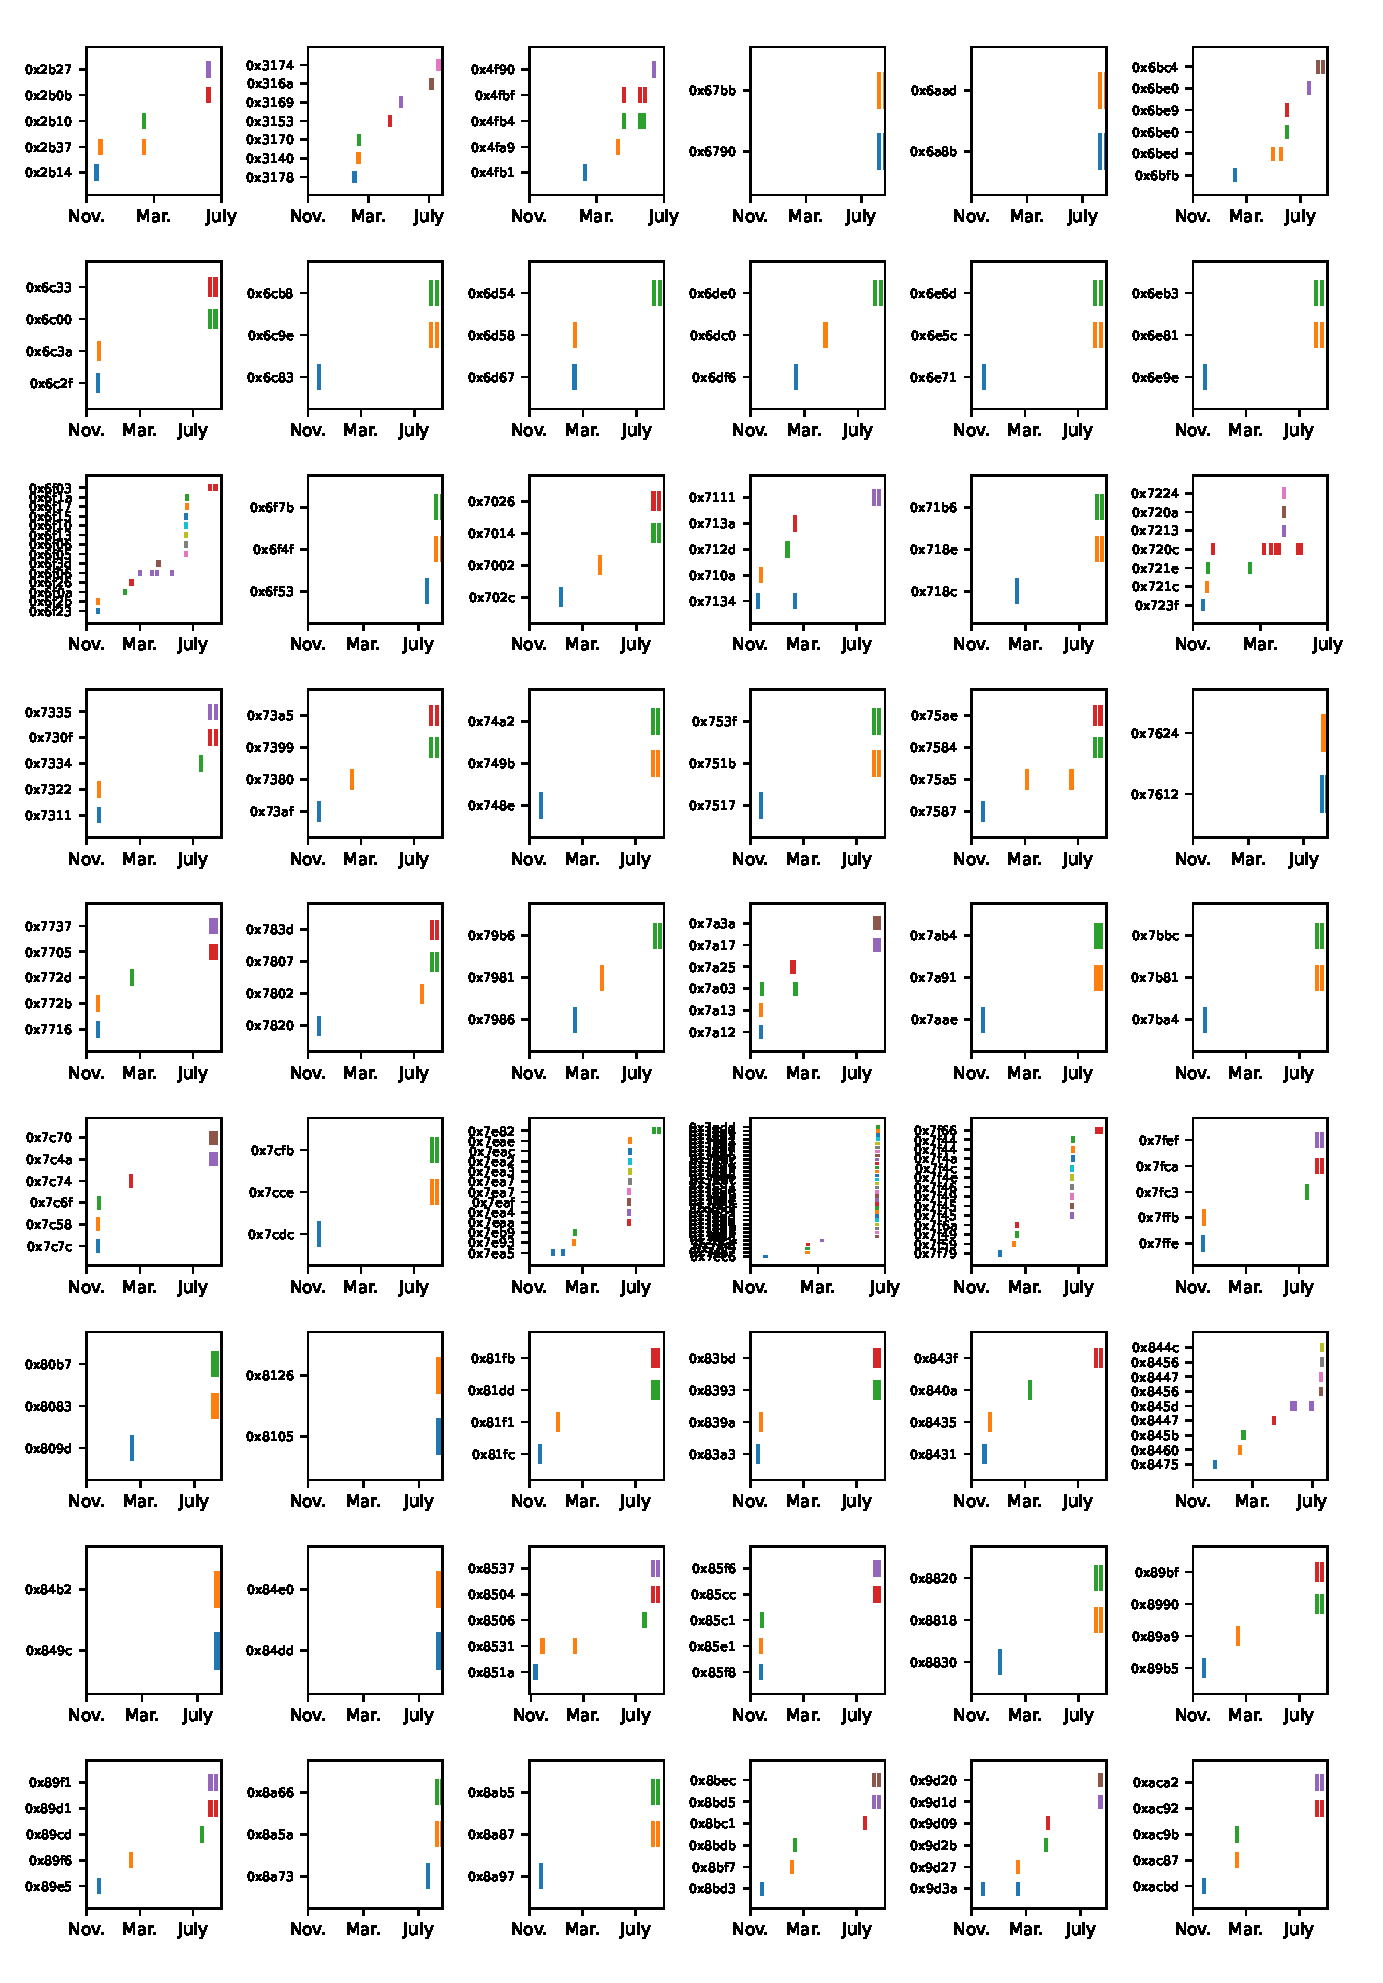
\includegraphics[width=\textwidth]{common/contested.eps}
%  \caption{Stake update events in contested neighbourhoods}
%  \label{event-plot}
%\end{figure}
%\end{center}


On many of the plots we can observe pairs of addresses that repeatedly top up at very similar times to one another.
%
We reproduce an example listing in Table \ref{event-listing}.
%
\begin{table}
\begin{tabular}{llr}
Date + time         & Address & Amount (BZZ) \\
\hline
2023-11-21 19:40:00 & 0x6c83 &   11 \\
2024-07-23 22:15:50 &	0x6c9e  &	10 \\
2024-07-23 22:16:05 &	0x6cb8  &	10 \\
2024-08-04 21:56:25 &	0x6c9e  &	10 \\
2024-08-04 21:56:45 &	0x6cb8  &	10
\end{tabular}
\caption{Event listing from in bin \code{0x6c8} --- cf.~the eighth plot in Figure \ref{event-plot}}
\label{event-listing}
\end{table}
%
We posit that the most likely reason for this behaviour is that the same entity started numerous nodes at the same time and placed them in distinct 11-bit neighbourhoods.
%
Since we have sorted by 10-bit neighbourhoods we have caught multiple of these nodes in the same bin, making their activity look like contention.

